\documentclass{sig-alternate}
\usepackage{verbatim}
\usepackage{array}
\usepackage{caption}
\usepackage{subcaption}
\usepackage{amsmath}
\usepackage{amssymb}
\usepackage{graphicx}
\usepackage{mathtools}
\usepackage[table]{xcolor}
\usepackage{xcolor,colortbl}
\usepackage{enumitem}
\usepackage{multirow}
\usepackage{tabularx}

\definecolor{myGray}{gray}{0.8}

%\newcommand\rankeq{\stackrel{\mathclap{\normalfont\mbox{rank}}}{=}}
\newcommand\rankeq{\mathrel{\overset{\makebox[0pt]{\mbox{\normalfont\tiny\sffamily rank}}}{=}}}

\setlist[itemize]{noitemsep}  % remove space between list items

\begin{document}

\numberofauthors{2}

\author{[Blind]}
%\author{
%Garrick Sherman and Miles Efron \\
%     \affaddr{Graduate School of Library and Information Science}\\
%       \affaddr{University of Illinois at Urbana-Champaign}\\
%       \email{\{gsherma2, mefron\}@illinois.edu}
%}
\conferenceinfo{CIKM}{2016 Indianapolis, Indiana, USA}

\title{Document knowledge base linking for information retrieval}

\maketitle
\begin{abstract}
Entity linking and wikification are the tasks of matching mentions of an entity, such as a person, place, or organization, or a concept with its representation in a knowledge base such as Wikipedia. While there has been some investigation into use of entity linking in information retrieval, its usage may be hampered by the computational expense of constructing accurate entity annotations on large corpora, the frequent need for training data to construct entity links, and the ambiguity involved in real-world entity linking. We present a method by which a ``bag of links'' from a document to a knowledge base may be generated using standard information retrieval techniques with Wikipedia. We also suggest a document expansion model that employs these links, which is effective in improving retrieval results.
\end{abstract}

% A category with the (minimum) three required fields
\category{H.3.3}{Information Search and Retrieval}{}

%\terms{}
%\keywords{Entity linking}

\section{Introduction}\label{section.intro}

Entity linking and wikification have been the subject of much research, spurred recently by the Text Analysis Conference (TAC) Knowledge Base Population (KBP) entity linking track. Systems are designed to link mentions of entities or concepts found in the text to their representations in a knowledge base such as Wikipedia\footnote{http://wikipedia.org} or Freebase\footnote{http://freebase.org}.

These links enrich documents by connecting knowledge base information such as hyperlink graphs, entity membership in categories, and additional text to the annotated documents. It seems reasonable that information retrieval (IR) systems might take advantage of this added source of information to improve the quality of search results. Unfortunately, producing high quality entity annotations is often a computationally expensive process. In addition, these systems generally require training data, which increases the barrier to use. Much entity linking and wikification research has also assumed more amenable circumstances that complicate their application to real-world text. For example, until 2014, the KBP entity linking track supplied explicit mention boundaries to participants.

For the purposes of ad hoc document retrieval, however, the granularity of linking entities to specific mention spans in the text is not necessarily required. Since retrieval is concerned with scoring documents in their entirety, we may simplify the task from mapping \textit{mentions} to entities, as is more common, to mapping \textit{documents} to entities. We argue that such a ``bag of links'' provides many of the same benefits as more fine-grained entity linking or wikification processes for the purposes of ad hoc document retrieval while improving computational efficiency and robustness against overfitting. This is because explicitly mentioned entities are often not directly related to the subject matter of documents: for example, a news article may explicitly mention the publisher of a book, which is less useful for document expansion purposes than unmentioned entities relating to the book's subject matter.

In this paper, we present a document expansion retrieval model to incorporate a ``bag of links'' into the document retrieval task. This model is in contrast to prior work applying entity links to IR, which has focused on \textit{query} expansion. Our document expansion model yields improvement over IR baselines.

\section{Related Work}\label{section.related}

\subsection{Entity Linking, Wikification, and Entity Retrieval}\label{section.related.entities}

Entity linking and wikification have been studied extensively, particularly in the context of TAC KBP \cite{Ji2014}. Entity linking systems often exploit knowledge base structure to help match and disambiguate entities. For example, Cucerzan \cite{Cucerzan2007} employs Wikipedia disambiguation pages and redirection pages to help identify various entity surface forms. Most systems employ some form of context, which often refers to the co-occurrence of entities as evidence for disambiguation \cite{Stoyanov2012, Dalton2013}. Alternatively, context may refer to the text surrounding an entity mention, which can be used to disambiguate knowledge base entries \cite{Mihalcea2007, Dalton2013}.

The related area of entity retrieval is also relevant to our work, e.g. \cite{Adafre2007, Bron2010}. Entity retrieval refers to the task of retrieving entities, rather than documents, in response to a specified information need. This was studied at the TREC entity retrieval track \cite{Balog2011}. Though entity retrieval tasks differ from ours in that entities are explicitly requested by the user, the querying of a corpus to retrieve entities is conceptually similar to much of our knowledge base linking approach.

\subsection{Document Expansion in IR}\label{section.related.ir}

Prior applications of knowledge base links in information retrieval use entity links in a feedback process for query expansion. Xiong and Croft, for example, employ FACC1\footnote{http://lemurproject.org/clueweb09/FACC1/} annotations on the document collection with supervised learning to expand queries \cite{Xiong2015}. Other researchers use entity links identified in query texts, rather than documents, to aid in expansion \cite{Xu2009, Brandao2014}. Still others use entity links in \textit{both} the query and documents \cite{Dalton2014, Li2015} to expand queries. Apart from entity linking, knowledge bases have also been used for query expansion in several related tasks, such as document filtering \cite{Xie2015} and blog search \cite{Elsas2008, Weerkamp2009}.

%Dalton and Dietz \cite{Dalton2014}, for example, use a number of sources, including entity-annotated queries and pseudo-relevance feedback (PRF) on entity-annotated document collections. Their process is underpinned by entity links produced by their own KB Bridge system \cite{Dalton2013}. Similarly, Xiong and Callan expand queries using pseudo-relevance feedback with the descriptions and categories of Freebase objects linked to a retrieved document in the FACC1\footnote{http://lemurproject.org/clueweb09/FACC1/} annotation data. They employ a supervised machine learning model to select expansion terms, trained on the basis of the terms' influence on the ranking scores of relevant documents \cite{Xiong2015}. Others, including \Li et al. expand queries using the Markov random field model for information retrieval using entity annotations in both the queries and the documents \cite{Li2015}. Other research has investigated query expansion with entities for closely related tasks, like filtering \cite{Xie2015}, entity annotations in the \textit{query}, rather than document \cite{Xu2009, Brandao2014}

In contrast, our approach is concerned with \textit{document} expansion. This expansion entails linearly interpolating the document language model with a second model estimated from the knowledge base links, discussed further in Section \ref{section.model}. Our idea is closely related to Wei and Croft's LDA-based document model, which smooths the document language model with latent Dirichlet allocation probabilities \cite{Wei2006}. Liu and Croft's \textit{CBDM} model performs a similar type of document expansion by interpolating the probability of a query term in a document cluster with its probability in the document \cite{Liu2004}.

\section{Constructing Knowledge Base Links}\label{section.linking}

\subsection{Underlying Retrieval Model}\label{section.linking.model}
Throughout this paper we rely on the language modeling retrieval framework \cite{Lafferty2001}, though this is not strictly necessary and imposes no particular mathematical constraints on our approach.

More specifically, our framework for all of the retrievals carried out in this work is the query likelihood (QL) ranking method.  Given a query $Q$ and a document $D$, we rank documents on $P(Q | \theta_D)$, where $\theta_D$ is the language model (typically a multinomial over the vocabulary $V$) that generated the text of document $D$.  Assuming independence among terms and a uniform distribution over documents, each document is scored by

\begin{flalign}\label{equation.ql}
\log P(Q | D) = \prod_{w \in Q} P(w | Q) \cdot \log P(w | \theta_D) .
\end{flalign}

\noindent We follow standard procedures for estimating the probabilities in Eq. \ref{equation.ql}.  We simply use the maximum likelihood estimate of $\hat{P}(w | Q) = \frac{c(w, Q)}{|Q|}$ where $c(w, Q)$ is the frequency of word $w$ in $Q$.  For $P(w | \theta_D)$ we estimate a smoothed language model by assuming that document language models
in a given collection have a Dirichlet prior distribution:

\begin{flalign}\label{equation.ql-dirichlet}
\hat{P}(w | \theta_D) = \frac{c(w, D) + \mu \hat{P}(w | C)}{|D| + \mu} 
\end{flalign}

\noindent where $\hat{P}(w | C)$ is the maximum likelihood estimate of the probability of seeing word $w$ in a ``background" collection $C$ (typically $C$ is the corpus from which $D$ is drawn), and $\mu \geq 0$ is the smoothing hyper-parameter. 


\subsection{Linking with Document Pseudo-Queries}\label{section.linking.queries}
%The KL-divergence retrieval model measures the distance between the query language model, $\theta_{D_Q}$ here, and the document language model, $\theta_E$, as follows:
%
%\begin{flalign*}
%	score(E,D_Q) 	&= -KL(\theta_{D_Q}||\theta_E) \\
%					&\rankeq \sum_{w \in V} P(w|\theta_{D_Q}) \log P(w|\theta_E)
%&\end{flalign*}
%
To find candidate entities to ``link" to a given document $D$, we begin by treating the text of $D$ as a pseudo-query which we pose against a collection of entities $C_E$.  To transform a document into a pseudo-query we apply two transformations.  First we remove all terms from $D$ that appear in the standard Indri stoplist\footnote{http://www.lemurpro ject.org/stopwords/stoplist.dft}.  Next, we prune our pseudo-query by retaining only the $0 < k \leq |D|$ most frequent words in the stopped text of $D$.  The integer variable $k$ is a parameter that we choose empirically.  Let $Q_D$ be the pseudo-query for $D$, consisting of the text of $D$ after our two transformations.

We obtain a list of candidate entities by running $Q_D$ over an index of our knowledge base, $C_E$, where each entry in this index is the text of an entity $E$'s knowledge base node. More formally, we rank the entities in our knowledge base against $D$ using Eq. \ref{equation.ql}, substituting $Q_D$ for the query and $E_i$---the text of the $i^{th}$ entity---for the document. Let $\pi_i$ be the log-probability for entity $E_i$ with respect to $D$ given by Eq. \ref{equation.ql}.  

We now have a ranked list of tuples $\{(E_1, \pi_1)$, $(E_2, \pi_2)$, $...$, $(E_N, \pi_N)\}$ relating knowledge base entry $E_i$ to $D$ with log-probability $\pi_i$. We take the top $n$ entries where $0 \leq n \leq N$. We call these top entries $\mathcal{E}_D$ and designate them as our knowledge base links for $D$.  Finally, we exponentiate each $\pi_i$ and normalize our entity scores so they sum to 1 over the $n$ retained entities.  Assuming a uniform prior over entities, we now have a probability distribution over our $n$ retained entities: $P(E | D)$.

Since this procedure does not depend on the query, we may compute $\mathcal{E}_D$ once at indexing time and reuse our knowledge base links across queries. 

\section{KB-Linked Retrieval Model}\label{section.model}

We would now like to incorporate our knowledge base links into a retrieval model over documents. Though many knowledge bases provide structured information such as hyperlink graphs and entity category information, in this work we focus only on the textual content supplied for each entry.

We assume that a query is generated by a mixture of the document language model $\theta_D$ and a language model $\theta_K$ representing the concepts linked from the knowledge base. We assume that $\theta_K$ can be estimated using the description texts of the linked knowledge base concepts $\mathcal{E}_D$. This mixture model may be expressed as:
%
\begin{flalign}\label{eq.ql-and-entities}
	\hat{P}^\lambda(Q|D) &= \prod_{i=1}^{|Q|} (1-\lambda) P(q_i|D) + \lambda P(q_i|\mathcal{E}_D)
\end{flalign}

\noindent The larger $\lambda$ is, the more we believe that the knowledge base concepts are responsible for generating $Q$, and the less we believe that the document is responsible for generating $Q$. We estimate $P(q_i|\mathcal{E}_D)$ in expectation:
%
\begin{flalign}\label{eq.entity-sum}
	P(q_i|\mathcal{E}_D) &= \sum_{E \in \mathcal{E}_D} P(q_i|E) P(E|D) .
\end{flalign}

\noindent Like $P(q_i|D)$, we estimate $P(q_i|E)$ as a Dirichlet-smoothed query likelihood, but using the description text for entry $E$ to estimate of the underlying model. By virtue of our entity-document scoring and normalization, we also have $P(E|D)$.

\section{Evaluation}\label{section.evaluation}

\subsection{Data}\label{section.evaluation.collections}

To perform knowledge base linking, we make use of the September 1, 2015 dump of English Wikipedia. We build an Indri\footnote{http://www.lemurproject.org/indri/} index over the Wikipedia page text. The text of each Wikipedia page also serves as the ``description text'' used in Eq. \ref{eq.entity-sum}.

We test our approach using the TREC 2004 robust topics. These 250 topics are used with data from TREC disks 4 and 5. In addition, we use the AP newswire collection from TREC disks 1 and 2 with topics 101-200. Using slightly older test collections helps to ensure that the knowledge base's coverage includes information about the topics; as noted in \cite{Frank2013}, updates to knowledge bases may lag considerably behind the occurrence of events.

For comparison, we also report the results of our model using entity links produced by Apache Stanbol\footnote{http://stanbol.apache.org/}. We process the test collections with Stanbol's default ``enhancer,'' which supplies entity links and corresponding confidence scores. Though Stanbol links to DBpedia\footnote{http://dbpedia.org} resources, these generally correspond to Wikipedia pages and may be converted easily. We select the link with the highest confidence for each mention in a given document and limit the set of links to $n$, the number of entities used in our bag-of-links approach. These links form the set of document links, and their confidence scores may be normalized to provide an estimate of $P(E|D)$.

\subsection{Runs}\label{section.evaluation.runs}

%In some of the following runs, we make use of the RM3 variant of relevance modeling \cite{Lavrenko2001} which interpolates the original query $Q$ with the relevance model using a mixing parameter $\alpha$. RM3 provides a stronger baseline than standard query likelihood.

We produce three runs per collection:
\begin{itemize}
	\item \textit{baseline-ql}, a baseline query likelihood run
%	\item \textit{baseline-rm3}, a baseline RM3 run
	\item \textit{kb-ql}, incorporating knowledge base links using Eq. \ref{eq.ql-and-entities}
	\item \textit{stanbol-ql}, which uses Stanbol entity annotations in place of our document-level links.
%	\item \textit{kb-rm3}, incorporating knowledge base links using an initial RM3 retrieval
\end{itemize}

We remove stop words in documents and entity descriptions for all runs. For the \textit{kb} and \textit{stanbol} runs, we retrieve the top 1000 documents per query based on the default Indri query likelihood implementation. We then re-rank these documents by incorporating their knowledge base links as described in Section \ref{section.model}.

\subsection{Parameters}\label{section.evaluation.parameters}

\begin{table}[htbp]
\centering
\begin{tabular}{|c|p{0.29\textwidth}|c|} \hline
{\bf Param} & {\bf Meaning} & {\bf Value} \\ \hline
$k$ & The maximum number of document terms to use in constructing $Q_D$. & 20 \\ \hline
$n$ & The maximum number of knowledge base entries in $\mathcal{E}_D$. & 10-100 \\ \hline
$\lambda$ & Mixing parameter controlling the weights of $P(q|D)$ and $P(q|E)$ & 0.0-1.0 \\ \hline
$\mu$ & Used for Dirichlet smoothing of both $P(q|D)$ and $P(q|E)$. & 2500 \\ \hline
%$fbDocs$ & The number of feedback documents to use for RM3 runs. & 20 \\ \hline
%$fbTerms$ & The number of terms per document to use for RM3 runs. & 20 \\ \hline
%$\alpha$ & Mixing parameter controlling the weights of the original query and relevance model for RM3 runs. & 0.5 \\ \hline
\end{tabular}
\caption{Parameter settings for the entity linking procedure and retrieval model}
\label{table.parameters}
\end{table}

The various parameters required for our approach, along with their meanings and the values used in our experiments, are shown in Table \ref{table.parameters}. 

We sweep across values of $\lambda$ and $n$ at intervals of 0.1 and 10 respectively to investigate the sensitivity of our model to these parameters. The results of these sweeps are shown in Figure \ref{figure.sweeps-ql} and discussed further in Section \ref{section.results}.

For this work, we set $k$ heuristically. In principle, this parameter need not be limited beyond the length of the document; however, this would increase computation time significantly, so we have opted to set it to the specified value.

\section{Results}\label{section.results}

\begin{table}[htbp]
\centering
\begin{tabular}{|c|l|c|c|c|} \hline
& {\bf Run} & {\bf $\lambda$} & {\bf $n$} & {\bf MAP} \\ \hline
\rule{0pt}{2.5ex} \multirow{3}{*}{Robust} & {\it baseline-ql} & -- & -- & 0.2183 \\ \cline{2-5}
\rule{0pt}{2.5ex} & {\it kb-ql} & 0.2 & 10 & 0.2354$^{\uparrow}$ \\ \cline{2-5}
\rule{0pt}{2.5ex} & {\it stanbol-ql} & 0.1 & -- & 0.2194 \\ \hline
\rule{0pt}{2.5ex} \multirow{3}{*}{AP} & {\it baseline-ql} & -- & -- & 0.2346 \\ \cline{2-5}
\rule{0pt}{2.5ex} & {\it kb-ql} & 0.2 & 20 & 0.2680$^{\uparrow}$ \\ \cline{2-5}
\rule{0pt}{2.5ex} & {\it stanbol-ql} & 0.1 & -- & 0.2355 \\ \hline
\end{tabular}
\caption{The top-scoring runs and baselines by MAP. Values marked with $\uparrow$ are statistically significant improvements over baselines.}
\label{table.performance}
\end{table}

\begin{figure*}
\centering
\begin{subfigure}{\columnwidth}
\centering
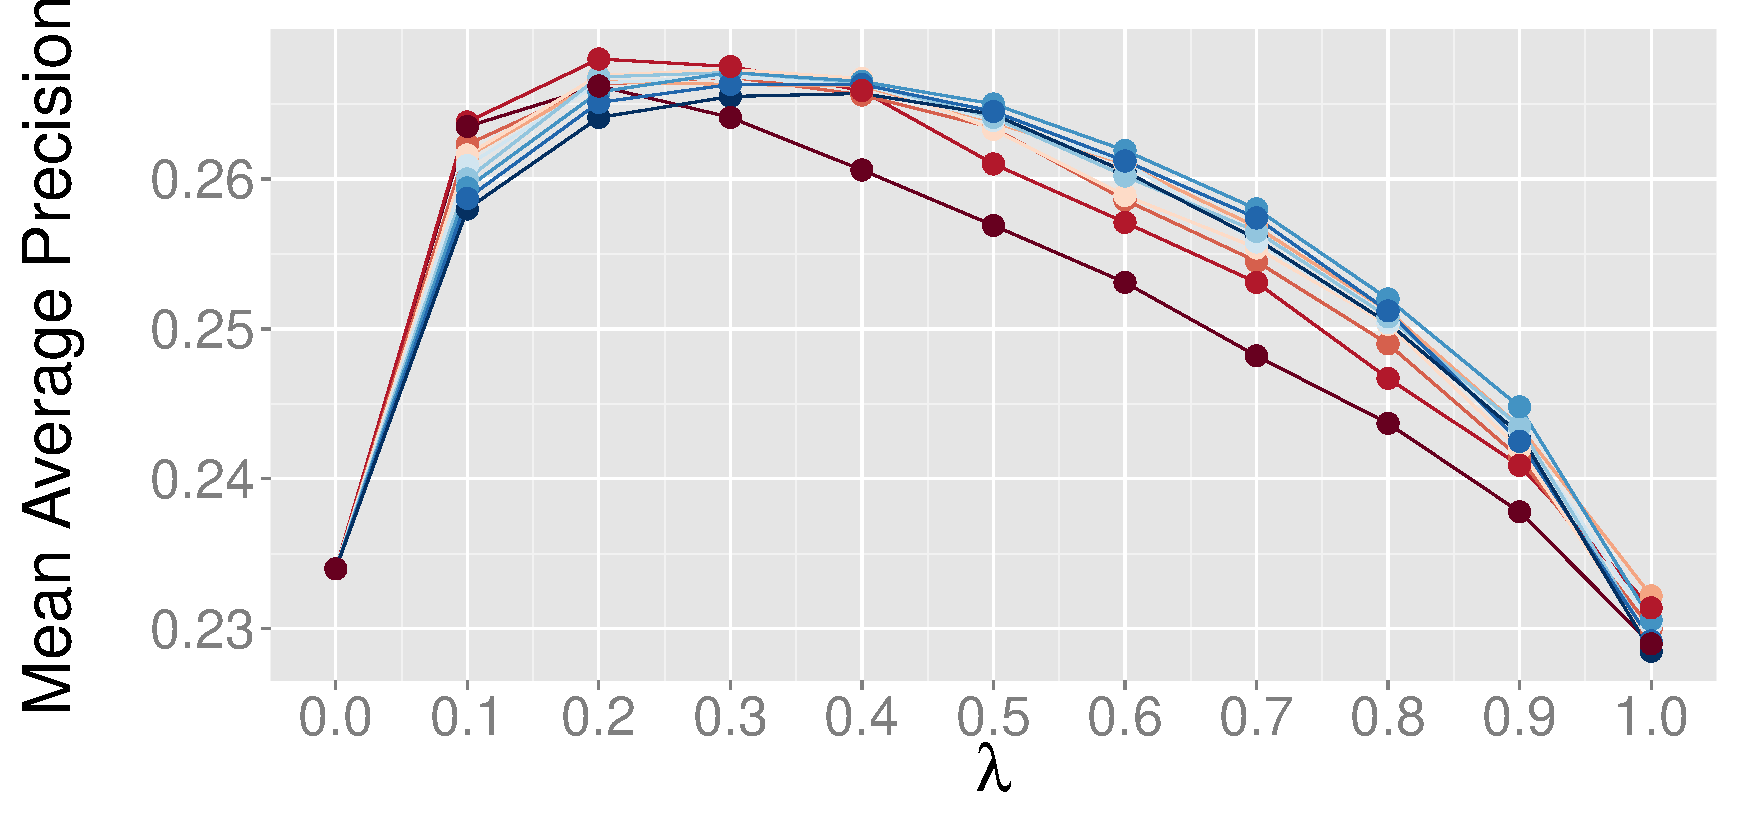
\includegraphics[width=\columnwidth]{figures/sweep-entities-AP.pdf}
\end{subfigure}%
\begin{subfigure}{\columnwidth}
\centering
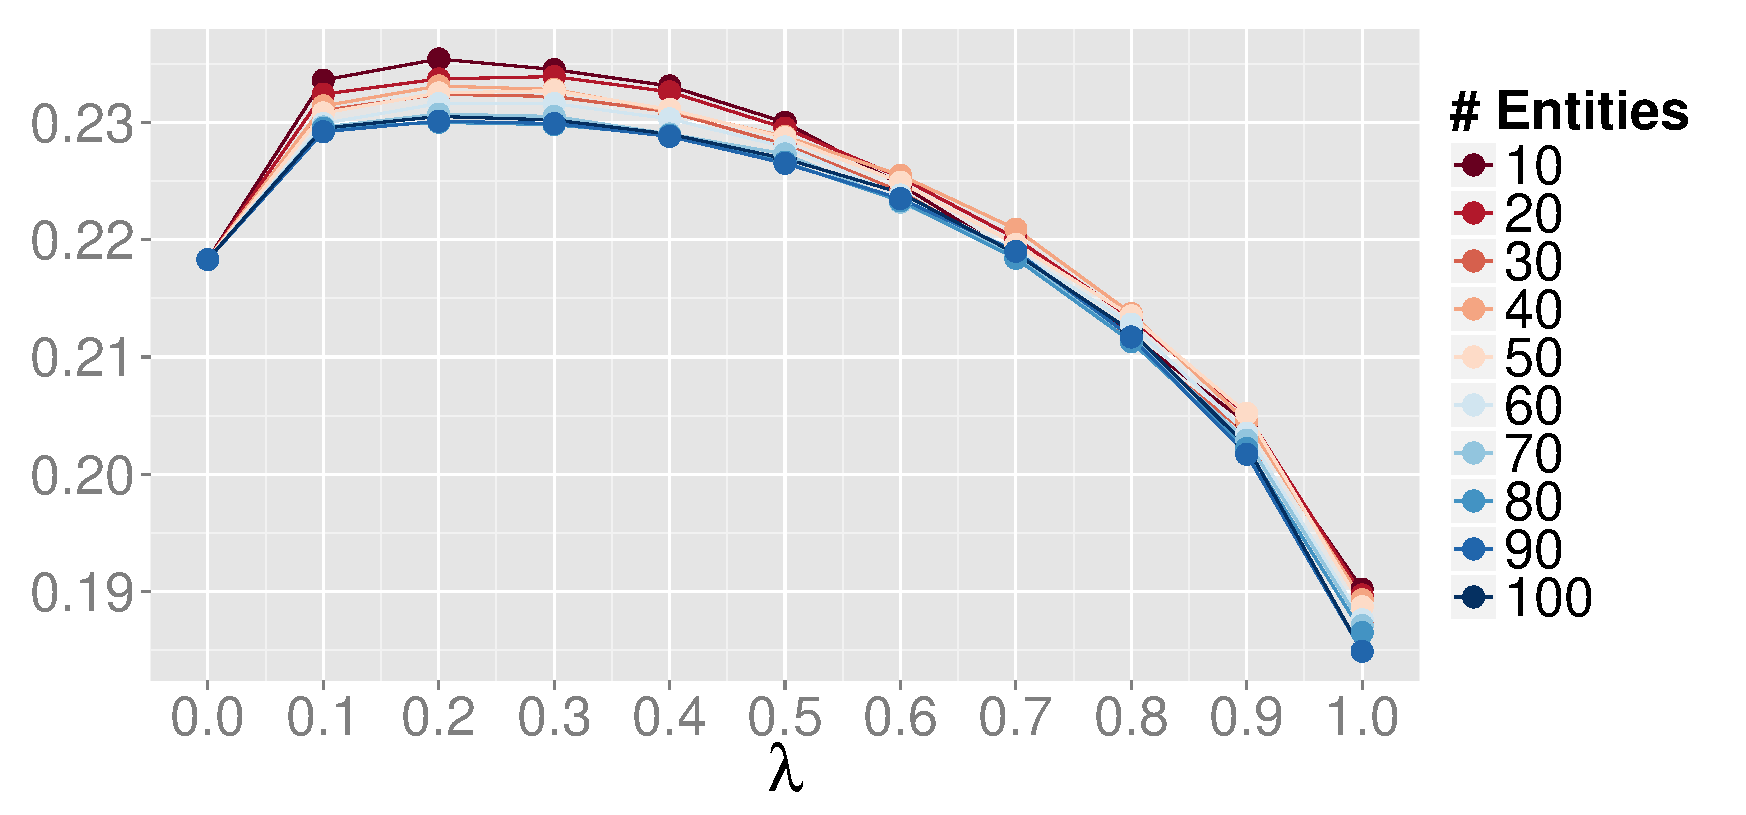
\includegraphics[width=\columnwidth]{figures/sweep-entities-robust.pdf}
\end{subfigure}
\caption{Sweeps over values of $\lambda$ for AP (a) and robust (b) runs. $\lambda=0.0$ is the baseline run scored only on the document text, while $lambda=1.0$ is based entirely on the entity text.}
\label{figure.sweeps-ql}
\end{figure*}

\begin{figure}
\centering
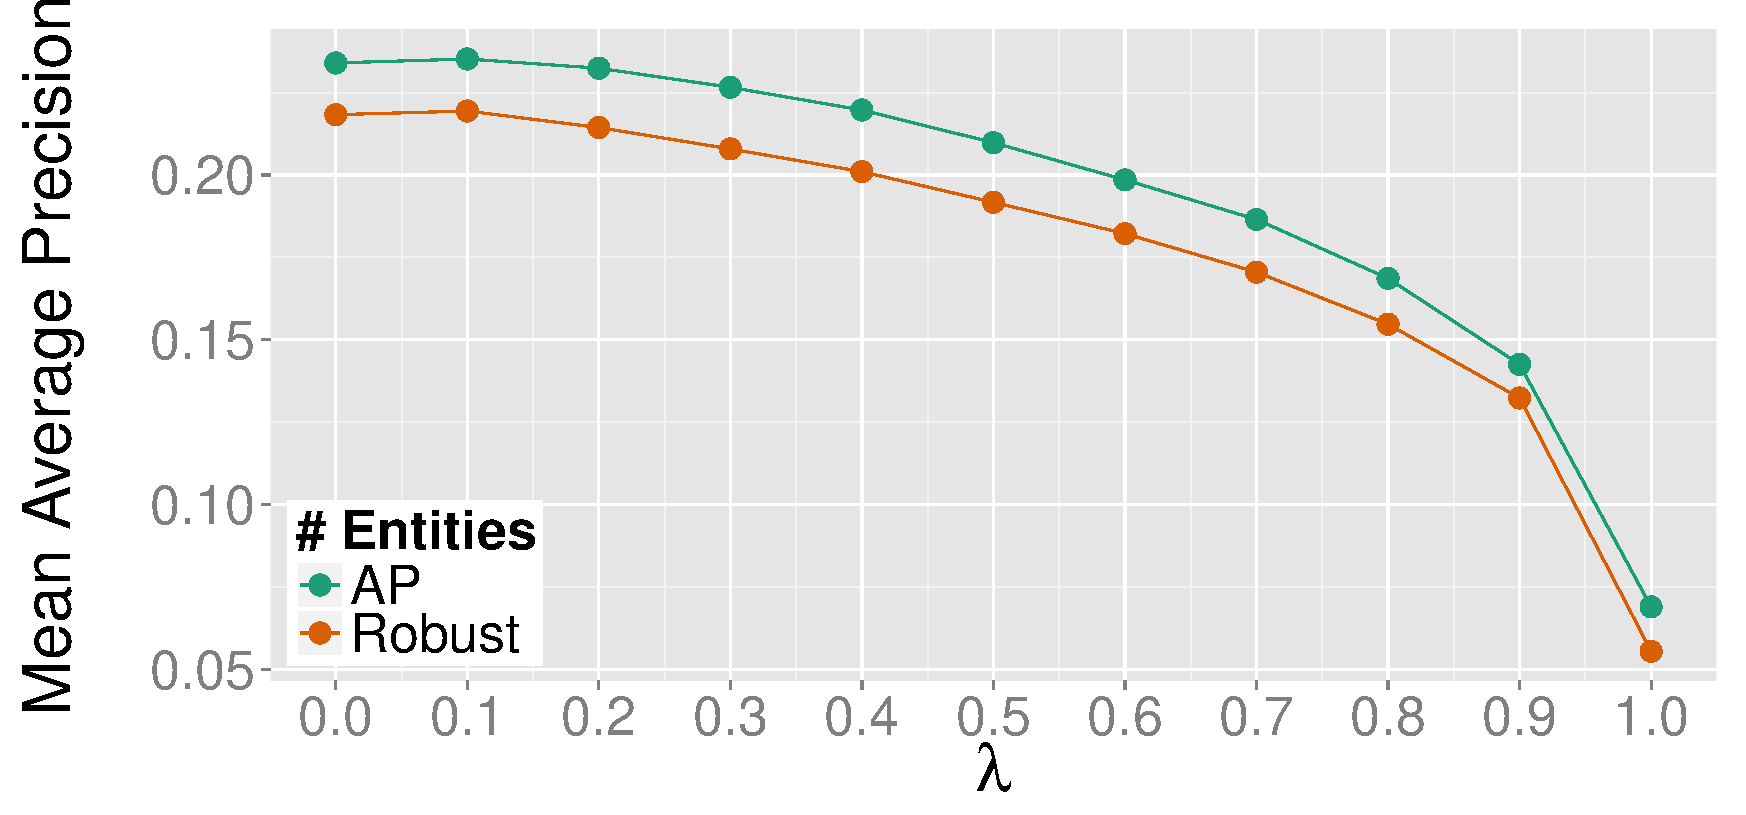
\includegraphics[width=.85\columnwidth]{figures/sweep-stanbol.pdf}
\caption{Sweeps over values of $\lambda$ for AP and robust \textit{stanbol} runs.}
\label{figure.sweeps-stanbol}
\end{figure}

Retrieval performance of the baselines and top-scoring runs are shown in Table \ref{table.performance}. Mean average precision (MAP) scores marked with $\uparrow$ are greater than the baseline run with statistical significance at $p < 0.05$ using a paired t-test. Note that baselines correspond to $\lambda = 0.0$. 

As Figure \ref{figure.sweeps-ql} shows, performance of \textit{kb} runs is not very sensitive to $n$, the number of linked entities. Though performance does vary somewhat based on $n$, a run's improvement or decline over the baseline depended only on the mixing parameter $\lambda$, with AP improving at $0.1 \leq \lambda \leq 0.9$ and robust at $0.1 \leq \lambda \leq 0.7$ for all values of $n$. Optimal performance for both collections occured at relatively small numbers of entities as shown in Table \ref{table.performance}; this is a convenient result since it allows for more efficient document expansion.

Notably, our model did not perform well when Stanbol annotations were used as a source of knowledge base links, as seen in Figure \ref{figure.sweeps-stanbol}. Both collections show very slight improvement at $\lambda = 0.1$, but this is not statistically significant and performance declines relative to the baseline at all other values of $\lambda$. We attribute this shortcoming to the overfitting of the Stanbol annotations to specific entity mentions in the text, rather than to concepts relevant to the document. Figure \ref{figure.sweeps-stanbol} does not present sweeps over $n$ for \textit{stanbol} runs because variations in performance at different values of $n$ are negligible using Stanbol entity links. This is due to the low number of linked entities produced by Stanbol: an average of 5.96 and 4.70 per document for AP and robust respectively.

\section{Conclusions}\label{section.conclusions}

The results indicate that our approach for constructing knowledge base links between documents and Wikipedia produces useful data for document retrieval purposes. Our simple document expansion model that incorporates these links performs well compared to a query likelihood baseline. These outcomes support our argument that a ``bag of links'' to a knowledge base can provide helpful information for a document retrieval task. Further, the poor performance of our model using more traditional mention-to-entity links indicates that not only are document-to-entity links more efficient to produce, they also connect more useful knowledge base entries for the purposes of document retrieval.

In this paper, we have limited ourselves to using only knowledge base description text. However, knowledge base links provide a great deal more information. Future work may benefit from harnessing this knowledge base data, including hyperlink graphs and entity categories. Since our retrieval model performs \textit{document} expansion, we also plan to investigate its utility when paired with \textit{query} expansion techniques that employ knowledge base links.

\section{Acknowledgments}\label{section.acknowledgments}
This work was supported in part by the US National Science Foundation under Grant No. [blind]. Any opinions, findings, conclusions, or recommendations expressed are those of the authors and do not necessarily reflect the views of the National Science Foundation.


\bibliographystyle{abbrv}
\bibliography{references}  




\end{document}
